% vim: tw=80

\chapter{The CMS Detector at the Large Hadron Collider}

The European Organization for Nuclear Research (\CERN) was founded in 1954.
Originally dedicated to the study of atomic nuclei, it is now devoted to the
research of sub-atomic particles and their interactions. To accomplish that
task, \CERN built several particle accelerators reaching record-breaking
energies and explored energy ranges not accessible before.

Ground-breaking achievements like the discovery of neutral currents in the
Gargamelle bubble chamber~\cite{Hasert:1973ff}, the discovery of the W and Z
boson by the UA1 and UA2 experiments~\cite{Arnison:1983rp} at the SPS
accelerator or the creation of antihydrogen atoms were made by physicists at
\CERN.

Remarkable insights into the Standard Model were gained by measurements at the
LEP accelerator at which the mass of the of the Z~boson and W~boson were
precisely measured. The proton-antiproton collider Tevatron at FNAL discovered
and measured the mass of the top quark accurately. Since the search for the long
anticipated higgs boson was unsuccesful due to their limited energy reach, an even
larger and more powerful accelerator was planned and built, the Large Hadron
Collider (LHC). The search for the higgs boson finally succeded in
2012~\cite{Chatrchyan:2012xdj}, but many further questions like the search for
supersymmetry or dark matter still need to be resolved in the future.

\section{The Large Hadron Collider}

The Large Hadron Collider (LHC) is the world's most powerful particle
accelerator and collider. The LHC is contained in the circular tunnel of the
preceding Large Electron Positron (LEP) collider which has a circumference of
\SI{27}{\kilo \meter} at a depth between \SI{50}{\meter} and \SI{175}{\meter}.
The tunnel crosses the border between Switzerland and France at four points and
two of the four main experiments are located in France. 

Two adjacent beamlines that intersect at four interactions points contain the
particle beams travelling in opposite directions. More than 1000 dipole magnets,
generating a magnetic field of up to \SI{8.3}{\tesla} bend the proton beams on
the circular track while almost 400 quadrupole magnets keep the beams focused. 

The proton beams are brought to collision at four interaction points which house
the LHC experiments ALICE~\cite{ALICE}, ATLAS~\cite{ATLASa}, CMS and
LHCb~\cite{LHCb}. ALICE is designed to study the quark-gluon plasma produced by
colliding heavy ions, which resembles the initial state of the universe. LHCB is
precisely measuring the CP violation and the decay of B mesons. ATLAS and CMS,
general purpose detectors allowing a broad field of phycis studies, were built
to search and study the Higgs boson and physics models beyond the standard
model. Additionally precision measurements of standard model predictions and
parameters improve the current knowledge and the confidence of predictions of
the standard model.

Prior to the injection and acceleration of protons in the LHC, the particles
pass a series of consecutive acceleration steps succesively increasing their
energy. The linear particle accelerator (LINAC2) generates \SI{50}{\mega
\electronvolt} protons, that
are further accelerated in the Proton-Synchrotron (PS) to \SI{26}{\giga
\electronvolt} and
the Super-Proton-Synchrotron (SPS) up to an energy of \SI{450}{\giga
\electronvolt}. At last the proton beams are injected into the LHC ring and are
further accelerated up to peak design energy of \SI{13}{\tera\electronvolt}. All these
pre-accelerators are not only used to feed the LHC, but also serve other physic
experiments as can be seen in Figure~\ref{fig:lhc_complex}.

\begin{figure}[htp]
    \centering
    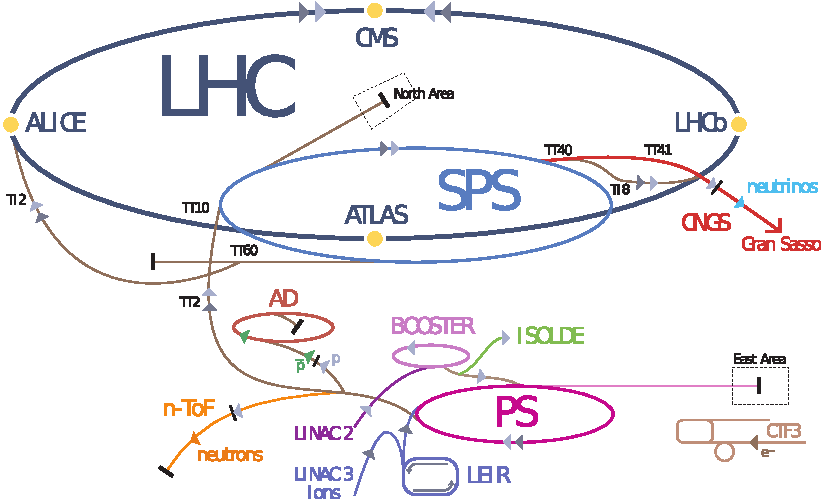
\includegraphics[width=0.8\textwidth]{figures/cms_detector/lhc_accelerator_chain.pdf}
    \caption[\CERN accelerator complex]{Several particle accelerators are
        chained together to feed proton beams into the LHC. Further experiments are
        located along the accelerator complex serving a broad program of physics
        studies~\cite{LHC:COMPLEX}.}
    \label{fig:lhc_complex}
\end{figure}

\section{Luminosity measurement}

The cross section $\sigma$ of a physical process is related to the
event rate $\dot{N}$ by the luminosity~$\mathcal{L}$

\begin{equation*}
    \dot{N} = \mathcal{L} \sigma.
\end{equation*}

The luminosity is dependent on the particle beam parameters and can be expressed
by

\begin{equation*}
    \mathcal{L} = = \frac{n_p^2
        n_b f_\mathrm{rev} \gamma F}{4 \pi \epsilon_n \beta^*}
\end{equation*}

where $n_p$ is the number of particles per bunch, $n_b$ the number of bunches
per beam, $f_\mathrm{rev}$ the revolution frequency, $\gamma$ the relativistic
gamma factor and $F$ the geometric luminosity reduction factor. The effective
collision area of the two beams is related to the normalized transverse beam
emittance $\epsilon_n$ and the value of the betatron function $\beta^*$ at the
interaction point.

The luminosity is constantly measured by the experiments. CMS employs two
methods to measure the relative instantaneous luminosity. The particle flux
measured in the hadron forward calorimeter is proportional to the instantaneous
luminosity. The second method counts the number of reconstructed vertices in the pixel
tracking detector. The results of both methods agree. The absolute luminosity
measurement is relying on van-der-Meer scans which are carried out in special
runs of the LHC~\cite{vanderMeer:296752}.

Fig.~\ref{fig:cms:lumi_integrated} shows the integrated luminosity delived by
LHC to the CMS experiments in the run periods from 2010 to 2012.

The uncertainty on the luminosity measurement for the 2012 LHC run is estimated
to 2.5\% (syst.) + 0.5\% (stat.)~\cite{CMS-PAS-LUM-13-001}. As it fully
propagates on any absolute cross section measurement, the uncertainty is later
on taken into account in the dijet cross section measurement.

\begin{figure}[h!tp]
    \centering
    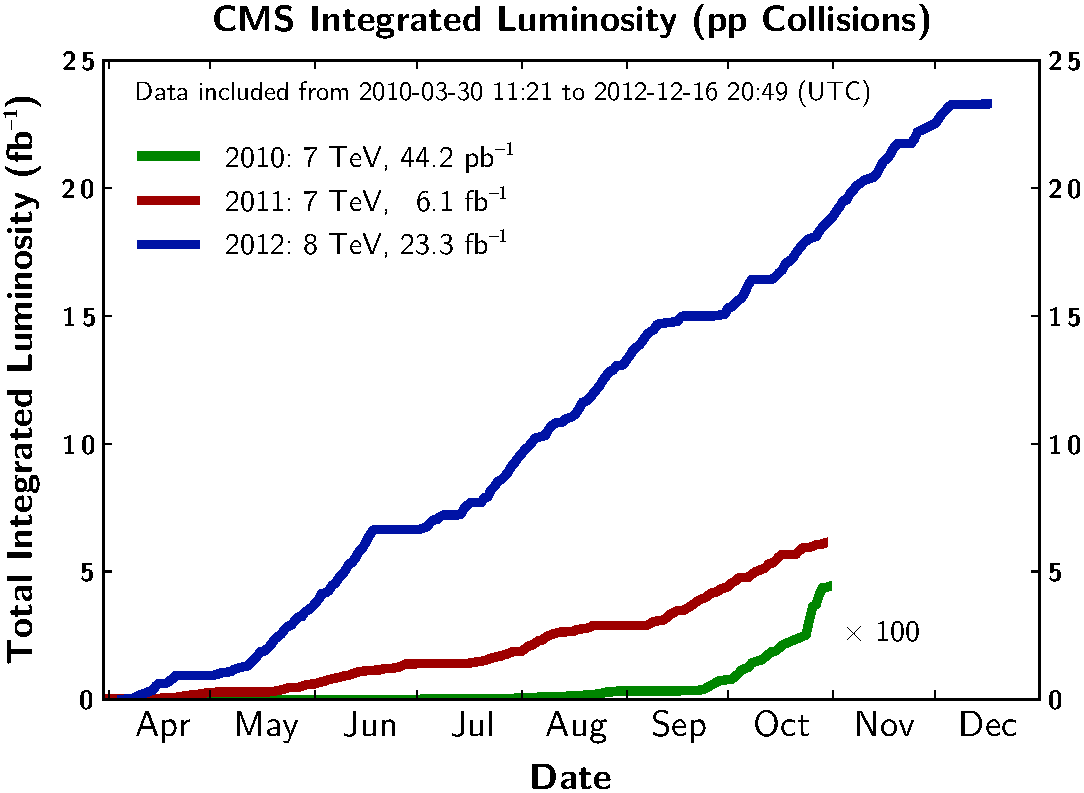
\includegraphics[width=0.8\textwidth]{figures/cms_detector/lumi_integrated.pdf}
    \caption[Integrated luminosity delivered to CMS]{Integrated luminosity
        delivered by the LHC to CMS in the 2010, 2011 and 2012 LHC run periods.
        Taken from~\cite{Berger:2014aca}.}
    \label{fig:cms:lumi_integrated}
\end{figure}


\section{The Compact Muon Solenoid Detector}

The Compact Muon Solenoid (CMS) detector is a general purpose detector at the
LHC, located at Point 5 of the LHC ring. To serve a wide range of physics
studies, the detector design is driven by a cylyndrical structure containing
layers of different subdetectors each built to measure a specific type of
particles with best precision. A high-precision inner tracking system is
surrounded by an electromagnetic and a hadronic calorimeter which again are
enclosed by a superconducting solenoid magnet. The whole inner part of the
detector is surrounded by a sophisticated muon detection system embedded in a
iron yoke. The detector is \SI{21.6}{\meter} long and \SI{14.6}{\meter} in
diameter, but weighing more than \SI{12000}{\tonne} due to its compact design.
It was built as cylyndrical slices constructed at ground level and lowered into
the cavern. In case of upgrades or repairs, the slices can be pulled apart and
the inner components can be easily accessed.

Fig.~\ref{fig:cms:longitudinal_section} shows a longitudinal section of one
quadrant of the CMS detector and the location of all subsystems.

The detector and physics performance of the CMS detector are discussed in
great detail in~\cite{Bayatian:922757,Ball:2007zza}. This section gives only a
short overview of the design and functional principles of the detector.

\begin{figure}[htp]
    \centering
    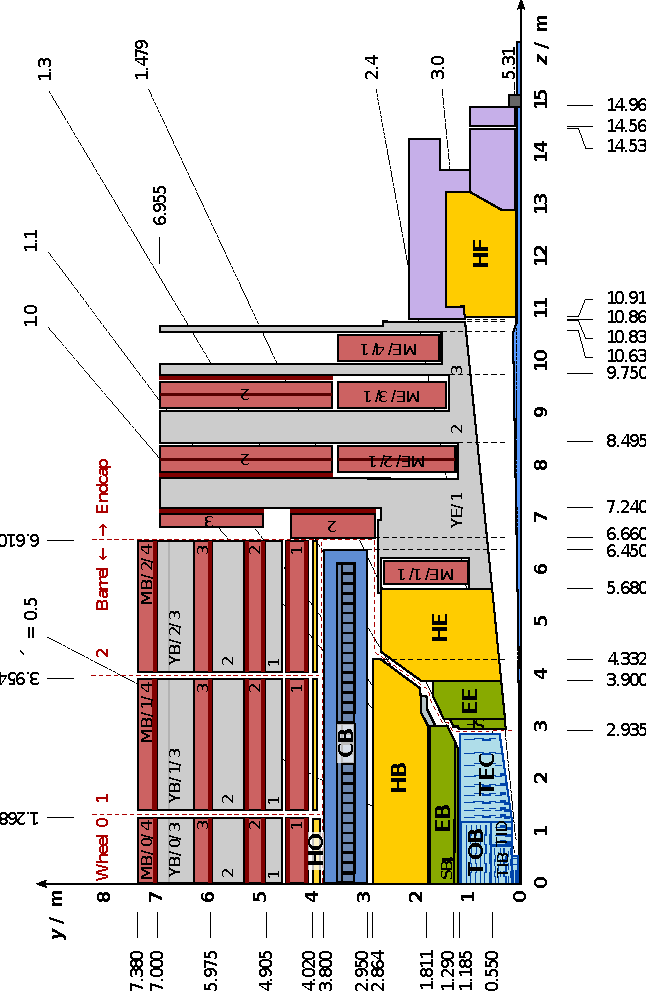
\includegraphics[width=0.8\textwidth]{figures/cms_detector/cms_longitudinal_section.pdf}
    \caption[Longitudinal section of the CMS
    detector]{A longitudinal section of one quadrant of the CMS
        detector in the $y$-$z$ plane. The sketch shows
    the multi-layer design of the CMS detector starting with the silicon pixel
and silicon strip detectors close to the interaction point. They are surrounded
by the electromagnetic (green) and hadronic (yellow) calorimeters. The barrel is
encompassed by the superconducting magnet (blue). The muon detection system
(red) is embedded in the iron return yoke~\cite{Berger:2014aca}.}
    \label{fig:cms:longitudinal_section}
\end{figure}

\subsection{Definition of the Coordinate System}

CMS uses a right-handed coordinate system centered at the nominal interaction point inside the
detector. The $x$-axis points radially inward towards the LHC ring centre, the
$y$-axis vertically upwards and the $z$-axis along the beam direction towards
the Jura mountains. Important quantities are the azimuthal angle $\phi$
measured from the $x$-axis in the $x$-$y$ plane and the polar angle $\theta$,
measured from the $z$-axis in the $z$-$y$ plane. Instead of the polar angle
$\theta$, the pseudo-rapidity $\eta$ and the rapidity $y$ are commonly used to
split the phasespace, since the differential flux is approximately constant at
hadron-hadron colliders. The pseudo-rapidity is defined as

\begin{equation*}
    \eta = - \ln \left( \tan \left( \frac{\theta}{2} \right) \right)
\end{equation*}

Throughout this thesis the rapidity is favoured compared to the pseudo-rapidity
due to its invariance under longitudinal boosts in the $z$-direction. Rapidity
and pseudo-rapidity are equivalent in the case of massless particles. The
rapidity is defined as

\begin{equation*}
    y = \frac{1}{2} \ln \left( \frac{E + p_z}{E - p_z} \right) 
\end{equation*}

The momentum along the beamline is not well defined due to the momentum
distribution inside the proton. A direct connection to the hard process is given
by the transverse momentum \pt related to cartesian coordinates as

\begin{equation*}
    \pt = \sqrt{p_x^2 + p_y^2}
\end{equation*}

\subsection{Inner Tracking System}

To yield a best possible spatial resolution, the particle tracks need to be
measured as close to the beam line as possible. The inner tracking system of CMS
consisting of silicon detectors is designed to measure the tracks of charged
particles emerging from the collision. A voltage is applied to the silicon
detectors to deplete them from free charges. As charged particles pass through
the detector material, they leave a small ionization currents which can be
measured and detected as a hit in the detector. By combining multiple hits, the
track of a charge particle can be reconstructed and the momentum and charge of
the particle determined. Due to the strong magnetic field of the CMS detector,
even tracks of particles with high transverse momenta have a measurable
curvature.
 
The inner tracking detector encloses the interaction point with a diameter of 2.6 m and
extends up to 2.8 m in each direction along the beampipe, the tracking system covers a
pseudo-rapidity range up to $|\eta| < 2.4$. The inner tracking system comprises
two subsystems, the silicon pixel detector consisting of three layers and
installed very close to the beam pipe and the silicon strip detector with ten
strip layers in the barrel region. 

\paragraph{Silicon Pixel Detector} Containing over \SI{65} milion pixels
arranged in three cylindrical layers at \SI{4}{\centi\meter},
\SI{7}{\centi\meter} and \SI{11}{\centi\meter} distance to the beam pipe, the
pixel detector is able to resolve the tracks of the huge number particles. At
LHC design luminosity, about 1000 particles pass the tracking detector on
average. The size of each pixel is \SI{100}{\micro \meter} x \SI{150}{\micro
\meter} giving a average occupancy of $10^{-4}$ per bunch crossing.  The high
spatial resolution achieved by the pixel detector additionally allows the
identification and measurement of secondary vertices used to identify long-lived
particles.

\paragraph{Silicon Strip Detector} The pixel detector is complemented by silicon
strip detector. Reduced particle flux further away from the beam pipe eases the identification
of tracks. Cost-efficient silicon strips are employed reaching out to
an radius of \SI{1.3}{\meter}. The strip detector consists of a total of 10 million
detecting strips read out by \SI{80000} chips. 

\begin{figure}[htp]
    \centering
    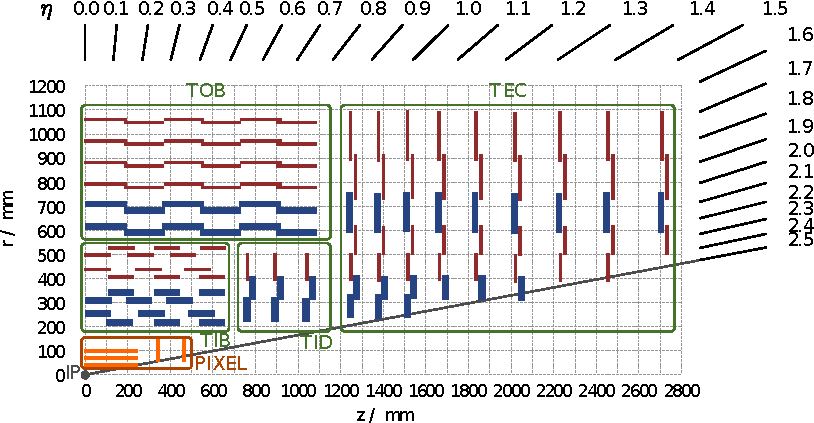
\includegraphics[width=0.65\textwidth]{figures/cms_detector/tracker.pdf}\hfill
    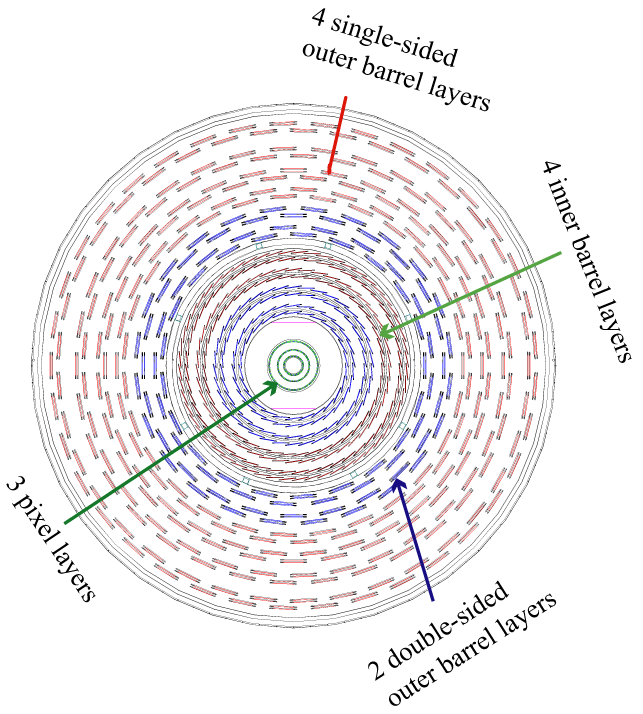
\includegraphics[width=0.3\textwidth]{figures/cms_detector/tracking_sytem_barrel_slice.png}
    \caption[Inner Tracking System]{The left figure shows one quadrant of the
        longitudinal section of the inner tracking system of CMS consisting of the
        silicon pixel detector and the silicon strip detector. The right figure shows a
        transverse section of the tracking system in the barrel region with overlapping
        arrangement of the strip modules. Figures taken
        from~\cite{Berger:2014aca} andi~\cite{cmsweb:innertracker}.}
    \label{fig:cms:inner_tracking}
\end{figure}

\subsection{Electromagnetic Calorimeter}

Measuring only the tracks of traversing particles is not sufficient to identify
the particles and derive their momentum. The energy needs to be measured as well
by stopping the particles in the detector and measuring the
deposited energy. The photon and electron energy is measured in the
electromagnetic calorimeter (ECAL). 

High-energetic photons, electrons or positrons which enter the dense material of
the ECAL detector, produce an electromagnetic shower via subsequent
bremsstrahlung and electron-pair production processes. Below a certain
threshold, the particles deposit their energy via compton scattering and the
photo-electric effect in the detector material resulting in an excitation of
the materials atomic state. When they return to ground state, they emit photons,
which are measured using avalanche photodiodes. The fraction of the deposited
energy is proportional to the number of emitted photons.

The hermetic calorimeter is made of lead tungstate ($\mathrm{PbWO}_4$), a very
dense material with a radiation length of $X_0 = \SI{0.89}{\centi\meter}$.
Through the additional oxygen, it is highly transparent and scintillates light.
The small Moli`ere  radius of \SI{2.19}{\centi\meter} leads to a fine granularity
These material properties allow the ECAL to be built very compact and to
be placed within solenoid magnet. 

\begin{figure}[htp]
    \centering
    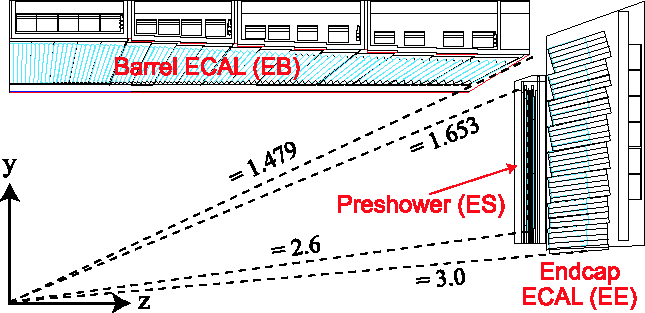
\includegraphics[width=0.8\textwidth]{figures/cms_detector/cms_ecal.pdf}\hfill
    \caption[Electromagnetic Calorimeter]{The electromagnetic calorimeter
    consists of two submodules covering the barrel region and the endcaps.
    An additional preshower detector is mounted in front of the
    endcaps. Taken from~\cite{cms:ecal}.}
    \label{fig:cms:ecal}
\end{figure}

Figure~\ref{fig:cms:ecal} shows a schematic sketch of the ECAL in the $y$-$z$
plane. The ECAL comprises three subsystems covering the the pseudo-rapidity
range up to 3.0. 

\paragraph{Electromagnetic Calorimeter Barrel (EB)} The EB covers up to $\eta <
1.479$ using more than 60000 crystals forming a homogenous coverage in
pseudo-rapidity. Each crystal measures $\SI{2.2}{\centi\meter} \times
\SI{2.2}{\centi\meter} \times \SI{23}{\centi\meter}$ corresponding to a
radiation length of 25.8 $X_0$.
\paragraph{Electromagnetic Calorimeter Endcaps
(EE)} It extend the pseudo rapidity coverage from $1.479 < |\eta| < 3.0$.  The
largest part of the ECAL endcap is additionally covered by the
\paragraph{Electromagnetic Pre-shower Detector (ES)}. It consists of two orthogonal
silicon strip sensors. The ES improves the discrimination between single
high-energetic photos and less interesting low-energy photon pairs as well as
the discrimination between neutral pions and photons.

The relative energy resolution of the ECAL can be parametrized using the NSC-formula

\begin{equation}
    \left( \frac{\sigma}{E} \right)^2 = \frac{N^2}{E^2} + \frac{S^2}{E} + C^2
\end{equation}

in which the first term describes the contribution by noise (N), the second
term the stochastic (S) component arising from the proportional relation between
the number of counted photons and the deposited energy and last a constant (C)
term.

\subsection{Hadronic Calorimeter}

Hadrons entering the calorimeter produce a hadronice shower. High-energetic
hadrons mostly shower in inelatic interactions producing a large number of pions
and nucleans. Due to the large transverse momentum of these secondary particles,
hadronic shower spread further in the calorimeter than electromagnetic shower.
When the energy of the particles involved in the shower drops below a certain
theshold, the energy is deposited by ionisation and low-energy hadronic
activity. The active scintillation material is excitated eand emits blue-violet
light. The scintillators are connected to photodiodes using wavelength
shifters which read out the signals and pass it to the data aquisition system.

The compact design of the CMS detector limits the size of the calorimeters. CMS
therefore built a sampling calorimeter inside the solenoid coil. The hadronic
calorimeter consists of brass as absorber material which is non-magnetic and
has a short interaction lenth of $\lambda_I = 16 \si{\centi\metre}$. It is
interleaved with plastic scintillators measuring the deposited energy. The CMS
hadronic calorimeter comprises three subsystems. 
\paragraph{Hadron Barrel Calorimeter (HB)}
It covers the barrel region up to a pseudo-rapidity $|\eta| <
1.305$. The absorbing material in the barrel has a corresponding thickness of
$5.39 \lambda$ in the central region up to $10.3 \lambda$ at $|\eta| = 1.3$. The
HB is complemented by the Hadron Outer Calorimeter (HO) located on top
of the coil of the magnet. Using the coil as absorbing material it is able to
meaure the tails of hadron showers penetrating the HB and the coil.

\paragraph{Hadron Endcap Calorimeter (HE)} The HE extends the pseudo-rapidity
coverage up to $|\eta| < 3.0$. A major challenge in the construction of the HE
were the usage of non-magnetic material to not disturb the magnetic field as
well as the close distance to the beampipe. Radiation damages decrease the
detector response and have to be corrected for continously. 

\paragraph{Hadron Forward Calorimeter (HF)} 
The forward calorimeter extends even closer to the beam pipe. With a coverage of
$2.8 < |\eta| < 5.2$ the calorimeter is adapted to the high radiation
environment. The HF is desinged using iron absorbers and quartz fibres as active
material, which measure the Cerenkov light emitted by the relativistic
components of the shower.

\subsection{Superconducting Solenoid}

A key component of the CMS detector is the superconductiong magnet which
produces a magnetic field of 4 T and is located inside the detector between the
calorimeters and the muon system. It measures a diameter of 6 m and a lenth of
12.5 m. When operated at design magnetic field strenth, the magnet contains an
energy of 2.6 GJ. The strong magnetic field is neccessary to bend the particle
tracks for a high momentum resolution in the tracking system. Operated at a
temperature of 4 K, the NbTi conductors become superconducting. The muon system
is installed within a 10,000 t iron yoke which return the magnetic field.

\subsection{Muon System}

Identifying and measuring muons with high precision is an unrivalled capacity of
the CMS detector. Unlike most other particles, muons are not stopped by the
calorimeters but leave the detector. Therefore, the muon system has been placed
around the other detector components to measure the bended tracks of the muons.

By combining the information of the inner tracking system and the muon
detectors, the path and the muon momentum can be measured precisely. The muon
system comprises three different types of detectors each suited for a specific
task. Drift tubes (DT) cover the barrel region up to $\eta < 1.2$, the endcaps
up to $\eta < 2.4$ are measured using cathode strip chambers (CSC) which also
work reliably in spatially varying magnetic field. The DT and CSC detectors
yield a precise spatial muon resolution. Both system are accompanied by
resistive plate chambers (RPC) which provide a fast response to the trigger
system.

\subsection{Trigger and Data Aquisition at CMS}

The LHC generates a huge number of collisions. At a beam crossing frequency of
\SI{25}{\nano \second}, there are 40 million bunch crossings per second with an
average of around 20 collisions per bunch crossing in the 2012 run era. With
todays available hardware, the storage of all collision data is not possible.
Furthermore, most of the collisions are soft and of low interest for physics
analyses. Therefore a complex trigger system consisting of a very fast
hardware-implemented component, the Level 1 trigger (L1) and a High Level
software trigger (HLT) analyze the events and accept only events which are
interesting for physics analyses.

\begin{figure}[htp]
    \centering
    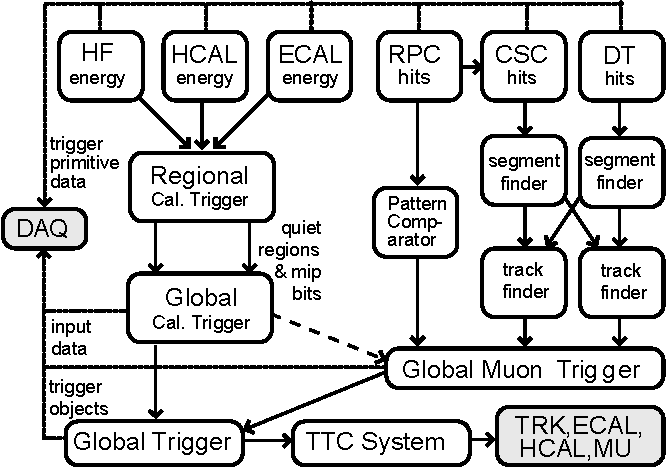
\includegraphics[width=0.8\textwidth]{figures/cms_detector/cms_l1_trigger.pdf}\hfill
    \caption[The L1 Trigger of CMS]{Workflow of the L1 trigger system. The
        regional triggers search for jets and compute the transverse and missing
        energy of an event. The global calorimeter trigger sorts the the objects
        from the regional calorimeter triggers and passes a part of the trigger
        obects to the Global triger, which accepts or rejects the event. If it
        is accepted, the complete data and the trigger objects are passed to the
        DAQ~\cite{Sphicas:2002gg}.}
    \label{fig:cms:l1_trigger}
\end{figure}

\paragraph{L1 Trigger} 
At the same frequency as collisions occur, the L1 trigger reads out the detector
electronics and analyzes the data using custom hardware. The workflow of the L1
trigger is shown in Fig.~\ref{fig:cms:l1_trigger}. Trigger Primitive Generators
calculate the transverse energy and missing energy from the frontend electronics
readout. Regional Calorimeter Triggers (RCT) identify electromagnetic showers
in the ECAL and sum up ECAL and HCAL trigger towers. Furthermore pattern
recognition is performed to identify jets and hadronic $\tau$ decays. A jet
candidate is defined that the transverse energy in a region o $4\times4$ trigger
towers is greater or equal to the transverse energy of the eight surrounding
regions, see Fig.~\ref{fig:cms:l1_calo_towers}. These
candidates are passed to the Global Calorimeter Trigger (GCT) which sorts the
incoming candidates from the all 18 regional triggers and passes the top
candidates to the Global Trigger (GT). The GT accepts events with a frequency
of \SI{100}{\kilo\hertz} and passes them to the data aquisition system, which
processes the data and transfers them to the HLT.

\begin{figure}[htp]
    \centering
    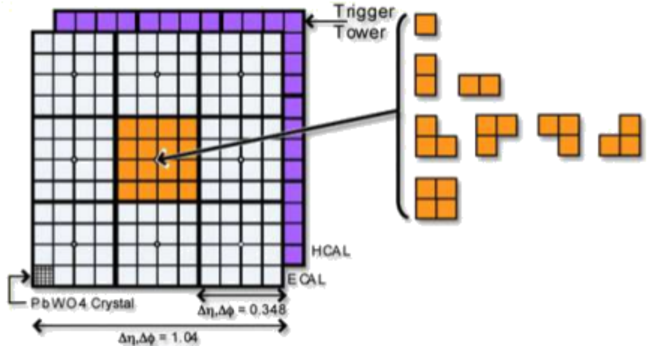
\includegraphics[width=0.8\textwidth]{figures/cms_detector/l1_calo_towers.pdf}\hfill
    \caption[Jet Candidates in the Level 1 calorimeter trigger]{Jet Candidates
        in the Level 1 calorimeter trigger ormed from $4\times4$ triger towers. Taken from~\cite{Rose:2009zz}.}
    \label{fig:cms:l1_calo_towers}
\end{figure}


\paragraph{HLT Trigger} The HLT is fully implemented in software running on a
dedicated computing farm at Point 5. The software is implemented in a
streamlined version of the CMS framework. Each HLT trigger path is a sequence of
reconstruction and selection steps with increasing complexity. The HLT selects
events a rate of several hundred Hertz which are grouped in non-exclusive data
streams, \eg the primpary physics stream \emph{A} or the calibration trigger
stream.

The HLT reconstructs jets using the \antikt clustering algrirthm. Because of the
high processing time of the particle flow algorithm, see
Sec.~\ref{sec:particle_flow_algorithm}, the jet trigger paths are divided into
multiple selection steps. At first the jets are reconstructed from calorimeter
towers.  Only for events in which at least one calorimeter jet passes a certain
\pt threshold, the particle flow algorithm is run and the jets are clustered
again from the particle flow candidates. Due to the flexibility of the HLT, it
is already possible to apply sophisticated jet energy corrections during the HLT
processing.

\paragraph{Data Aquisition (DAQ)}

As the L1 trigger accepts events at a rate of \SI{100}{\kilo\hertz}, the DAQ
system has to process the events at the same speed. It reads out the data of all
detector subcomponents and assembles the whole events, see
Fig.~\ref{fig:cms:daq_system}. The data is subsequently passed to the HLT
trigger which further reduces the rates to a few hundred events per second.
These events are then merged and saved on a storage system from which they are
transferred to the Tier 0 computing center at \CERN 

\begin{figure}[h!tp]
    \centering
    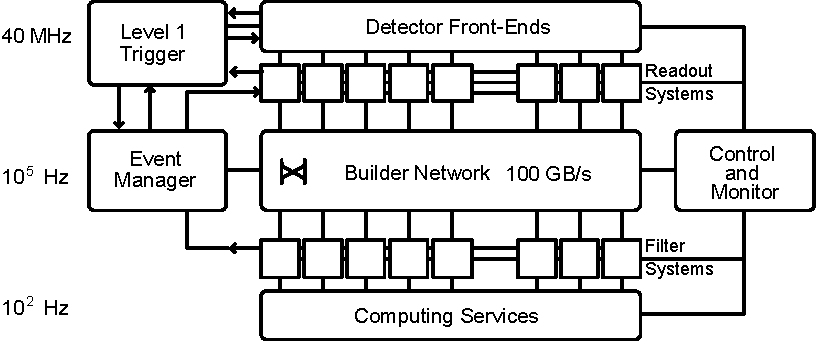
\includegraphics[width=0.8\textwidth]{figures/cms_detector/cms_daq.pdf}\hfill
    \caption[The DAQ System of CMS]{asdf~\cite{Sphicas:2002gg}}
    \label{fig:cms:daq_system}
\end{figure}

\section{Computing Infrastructure and Software Tools}

The vast amount of and the complexity of the data produced at the LHC
experiments poses many challenges for the computing infrastructure and the
engaged software. On the theory side, powerful Monte-Carlo event generators need to be
developed which are able to simulate the collision events. On the experimental
side, the raw detector the physical event information needs to be reconstructed. Additionally the
complex architecture of the detector response needs to be modelled and
simulated. These central tasks are approached using a common software framework
within CMS, the \CMSSW framework, which interfaces the various theory tools and
all the reconstruction and detector software. All of these tasks are divided
into smaller processing tasks, called jobs, which are assigned to computing
centers distributed over many countries. This common computing and storage
infrastructure is called the worldwide LHC computing grid (LHCG).

\subsection{Worldwide LHC Computing Grid}
\todo{write}

To overcome the discussed challenges and ease the access of users to the data of
the LHC experiments, a distributed grid with a tiered infrastructure was
developed. As the majority of the data is produced at \CERN, a hierarchical
structure with the computing center at \CERN, called Tier-0 at the top was
chosen, see Fig.~\ref{fig:lhc_tier_structure}. The raw data is stored at \CERN
and distributed to globally distributed Tier-1 centers, as they provided further
storage resources and large computing resources for the reconstruction and
analysis of the data. Tier-2 sites provide additional computing ressources while
Tier-3 sites are mostly used by local analysis groups for data analyses.

\begin{figure}[htp]
    \centering
    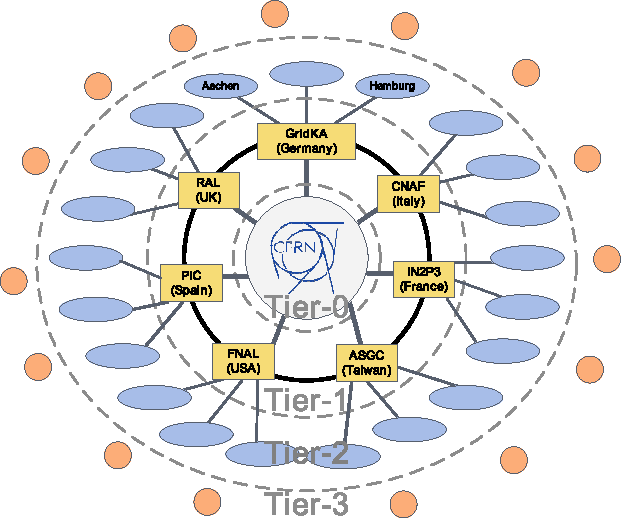
\includegraphics[width=0.8\textwidth]{figures/cms_detector/lhcg.pdf}\hfill
    \caption[Tiered structure of the worldwide LHC Computing Grid]{The WLCG is
        ordered hierarchical with the \CERN T0 at the top. Taken
        from~\cite{Stober:2012abc}.}
    \label{fig:lhc_tier_structure}
\end{figure}

Access to the ressources of the WLCG is gained by certificates, which authorize
the user to access the storage and computing resources.


\subsection{CMS Software Framework}

The software framework of the CMS collaboration, referred to as \CMSSW, offers
all neccessary tools for a phycis analysis. The tasks in the event processing
comprise on the one hand calibration and reconstruction of data from raw
detector read out and on the other hand the event generation and detector
simulation. Furthermore it provides the possibility to implement analysis code
to perform the data analysis. 

To cope with this vast range of requirements to the experiment software, \CMSSW
is built on top of an event data model (EDM) in which the event is a
container for for all measured or simulated data. The reconstruction and
distribution algorithms in \CMSSW are divided into modules, which can be
modularly loaded and run. Each module can read the event data and add additional
objects calculated within the algorithm. The execution of the modules is ordered
in processing chains which are configured by the user. Very often these modules
access external libraries like Monte Carlo event generators for event
simulation, Geant 4 for the detector simulation or FastJet for the
reconstruction of jets. Using this modular approach in which modules are loaded
dynamically one can easily start with an event containing only the raw detector
data and process all neccessary steps to arrive at the final event containing
the reconstructed objects suited for analysis.

While having that much information in the event data is convenient to redo
reconstruction steps, it is unsuited for fast processing in the analysis due to
its size and complexity. Therefore a skimming step, in which only the neccesary
data is preserved is run before the analysis, see Section~\ref{artus_kappa}.

\subsection{Analysis Software and Workflow}

Due to the complexity of the workflows in the HEP data analysis, several tools
were used or even deloped in the Karlsruhe group to faciliate a reliable and
fast workflow for the analysis. 

\subsubsection{Artus and Kappa}
\label{artus_kappa}

The Kappa software is a skimming framework interfaced to \CMSSW. It consists of
different modules which allow to skim only the physics objects needed in the
subsequent analysis. The data is then stored in its own compact data format
using the ROOT format. The resulting Kappa tuples provide all neccesary
information of the events and the lumisection while hiding the complexity of the
\CMSSW datasets. There is a separate tool collection, KappaTools, in which
functions to access the Jet energy corrections or HLT informations are
collected.

\begin{figure}[htp]
    \centering
    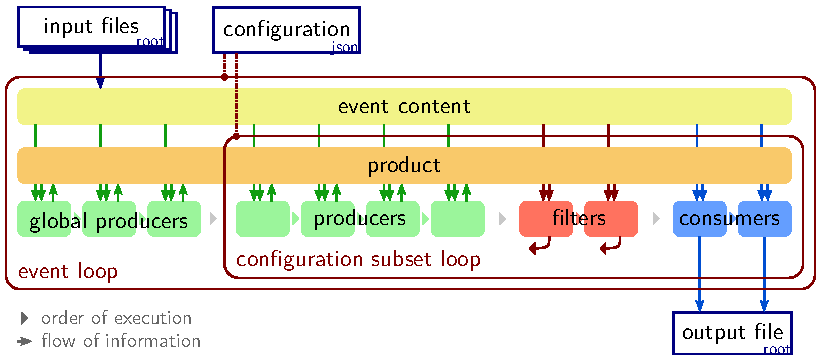
\includegraphics[width=0.8\textwidth]{figures/cms_detector/artus_workflow.pdf}
    \caption[Workflow of an analysis in the Artus framework]{Workflow of an
        analysis in the Artus analysis framework. Taken
        from~\cite{Berger:2014aca}.}
    \label{fig:artus_workflow}
\end{figure}

The analysis itself is built on top of the Artus framework. Artus was developed
within the Karlsruhe group to combine analysis efforts and profit from mutual
developments. The framework defines a workflow based on three elements. There
are \emph{producers}, which calculate quantities and \emph{filters}, which
reject events based on the defined criteria. In a final step, histograms or
nTuples are written out by \emph{consumers}. All producers, filters and
consumers are written in a modular way so that they can be shared with other
analyses. Furthermore they are steered by a global configuration file in which
one can easily adapt all settings and cuts.

\subsubsection{grid-control}

The data sets are even after the skimming step to large to be processed on a
single computer. Therefore special batch system with a huge number of computing
nodes are employed to process the data. The data processing is split into
multiple jobs which are then sent to the batch system. grid-control is by far
the most versatile job submission tool which provides multiple options for data
splitting and parametrized jobs while hiding the pitfalls of local or remote
computing resources.

\subsubsection{ROOT}

The object-oriented data analysis framework ROOT has been written almost 20 years
ago. It is used by all LHC experiments for persistent storage of data. Moreover
ith provides fast histogramming classes and access to many libraries like MINUIT
for minimization purposes or TMVA for multivariate data analyses. Despite
many hours of headaches caused by obscure design decisions in the software, ROOT
and especially the python bindings PyROOT were used extensively in this analysis.

\subsubsection{matplotlib and numpy}

matplotlib is 2D plotting library written in the python programming language~\cite{Hunter:2007aa}. It
provides publication quality plots in a variety of output formats and is very
pleasant to use. All plots in this thesis were made using matplotlib. The
plotting library matplotlib as well as many scripts used in this thesis rely on
the scientific computing library NumPy~\cite{Oliphant:2007aa}. NumPy provides
powerful n-dimensional arrays and tools to manipulate them. 

\subsection{Monte-Carlo Event Generators and Simulation Software}
\label{subsection:mc_generators}

\subsubsection{Pythia}

The multi-purpose event generator Pythia simulates events in high-energy
collisons, comprising a large set of physics processes. Pythia uses the Lund
string hadronization model in which all but the highest-energy gluons are
treated as field ines which attract each other by gluon self-interaction and
form a tube or string of strong color field. In this analysis two version of the
Pythia event generator are used. The official samples including the detector
simulation were generated using Madgraph and Pythia 6, while the study of
non-perturbative effects was performed using the new Pythia 8 version, in which
all the new tunes were available. 

\subsubsection{Herwig}

Herwig is also a multi purpose event generator for the simulation of high-energy
hadron-hadron collisions. The first version was build in Fortran and is known as
HERWIG~\cite{Corcella:2000bw}. Herwig++~\cite{Bahr:2008pv} builds up on the
heritage of the HERWIG version while providing a much more flexible structure as
it is implemented in C++. The recently released Herwig~7~\cite{Bellm:2015jjp}
version combines all their developments and supersedes both version. 

The Herwig generator family includes all steps to simulate events. It includes a
number of hard scattering processes, but also possesses the possibility to
interface external matrix element generators. The parton shower simulates
initial- and final-state radiation via angular ordering, multiple partonic
scatterings are simulated by an eikonal model and a cluster model decribes the
hadronization. 

Herwig 7 further improves these capabilities by including next-to-leading order
QCD matrix elements with matched parton showers while keeping the key features
of the previous Herwig versions. Herwig++ is used in this thesis to study
non-perturbative effects, see Sec.~\ref{sec:np_factors}. The NLO capabilities of
Herwig 7 are shown in the comparison of the unfolded measurement to NLO
predictions with matched parton showers, see Sec.~\ref{sec:nlo_comparisons}.

\subsubsection{MadGraph}

MadGraph is a multi-purpose tree-element matrix element generator. It implements
a large number of processes and can be interfaced to Monte Carlo Event
generators. In this thesis the MadGraph matrix elements are used together with
the Pythia 6 event generator for general comparisons to data.

\subsubsection{NLOJet++ and fastNLO}
\label{sec:nlojetpp}

% To populate the whole accessible phasespace with sufficient events to get a
% precise prediction, a huge number of events is neccessary. Since especially the
% influence of the PDFs and the strong coupling constant is interesting to be
% studied, the calculation would have to be repeated multiple times with different
% input parameters. In order to speed-up this process, \NLOJETPP is interfaced to
% the \fastNLO package~\cite{Kluge:2006xs,Britzger:2012bs}. fastNLO uses
% sophisticated interpolation tables to store the matrix element coefficients as a
% function of the scales, the calculation order and the fractional proton
% momentum. The fastNLO tables can now be evaluated with different PDFs, \as and
% scales within negligible time. 


The complicated NLO cross section for jet productions are calculated using
\NLOJETPP. It implements the dipole subtraction method for the separation of the
divergences. \NLOJETPP can calulate up to three-jet observables at NLO precision.
It implements the ability run analysis scenarios by which it is interfaced to
\fastNLO.

Since the pQCD cross section calculations in \NLOJETPP are determined in Monte
Carlo integration and are therefore very time consuming. For fits of the proton
structure or the extraction of the stroung coupling constant, the cross sections
need to be evaluated multiple times with different input parameters. The
\fastNLO framework implements a strategy for a fast recalculation of these cross
section. It sotres the perturbative coefficients obtained with \NLOJETPP in a
way that the strong coupling constant and the PDFs can be changed afterwards
without a recalculation of the perturbative coefficients.

\subsubsection{LHAPDF}

All event generators and cross section calculation tools need the parton
distribution functions as input. They are either hardcode in the generator or
accessed using a standardized interface, the LHAPDF library. LHAPDF provides
interpolation routines by which PDFs read from discretised data files can be
accessed. 
